\documentclass[tikz, border=2pt]{standalone}
\usetikzlibrary{positioning, arrows.meta, shapes, calc, fit, babel}
\usepackage{helvet}
\renewcommand{\familydefault}{\sfdefault}
\begin{document}
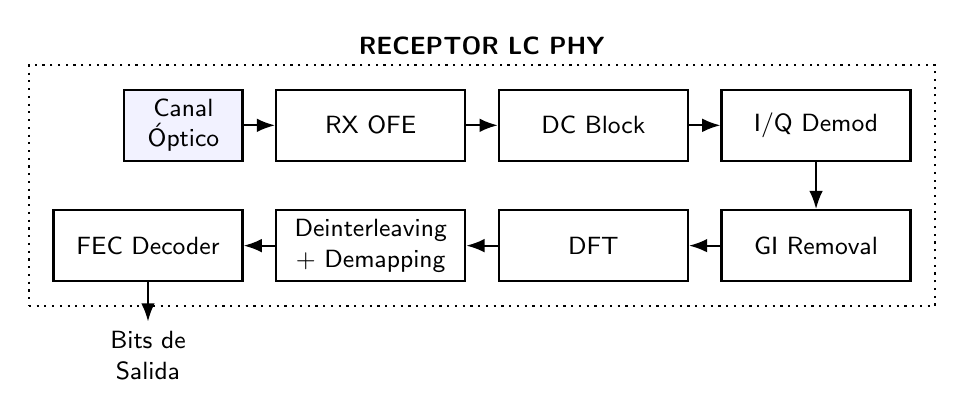
\begin{tikzpicture}[>=latex, font=\small, 
	block/.style={draw, thick, minimum height=0.9cm, minimum width=2.4cm, align=center, fill=white},
	smallblock/.style={draw, thick, minimum height=0.9cm, minimum width=1.5cm, align=center, fill=white},
	arrow/.style={-Latex, thick}]
	
	\node[smallblock, fill=blue!5] (channel_rx) {Canal\\Óptico};
	\node[block, right=0.4cm of channel_rx] (ofe_rx) {RX OFE};
	\node[block, right=0.4cm of ofe_rx] (dc_rx) {DC Block};
	\node[block, right=0.4cm of dc_rx] (iq_rx) {I/Q Demod};
	
	\node[block, below=0.6cm of iq_rx] (gi_rx) {GI Removal};
	\node[block, left=0.4cm of gi_rx] (dft_rx) {DFT};
	\node[block, left=0.4cm of dft_rx] (deint_rx) {Deinterleaving\\+ Demapping};
	\node[block, left=0.4cm of deint_rx] (fec_rx) {FEC Decoder};
	
	\draw[arrow] (channel_rx) -- (ofe_rx);
	\draw[arrow] (ofe_rx) -- (dc_rx);
	\draw[arrow] (dc_rx) -- (iq_rx);
	
	% Conexión hacia abajo de Fila 1 a Fila 2
	\draw[arrow] (iq_rx) -- (gi_rx);
	
	\draw[arrow] (gi_rx) -- (dft_rx);
	\draw[arrow] (dft_rx) -- (deint_rx);
	\draw[arrow] (deint_rx) -- (fec_rx);
	
	\node[below=0.5cm of fec_rx, align=center] (output) {Bits de\\Salida};
	\draw[arrow] (fec_rx) -- (output);
	
	\node[draw, dotted, thick, inner sep=0.3cm, label={above:\textbf{RECEPTOR LC PHY}}] 
	(rx_box) [fit=(channel_rx) (iq_rx) (gi_rx) (fec_rx)] {};
\end{tikzpicture}
\end{document}
